%%%%%%%%%%%%%%%%%%%%%%%%%%%%%%%%%%%%%%%%%
% Beamer Presentation
% LaTeX Template
% Version 1.0 (10/11/12)
%
% This template has been downloaded from:
% http://www.LaTeXTemplates.com
%
% License:
% CC BY-NC-SA 3.0 (http://creativecommons.org/licenses/by-nc-sa/3.0/)
%
%%%%%%%%%%%%%%%%%%%%%%%%%%%%%%%%%%%%%%%%%

%----------------------------------------------------------------------------------------
%	PACKAGES AND THEMES
%----------------------------------------------------------------------------------------

\documentclass[UTF8,aspectratio=169,14pt]{ctexbeamer}

\usepackage{hyperref}
\hypersetup{
	colorlinks=true,
	linkcolor=red,
	anchorcolor=blue,
	citecolor=green
}

\mode<presentation> {
	
	% The Beamer class comes with a number of default slide themes
	% which change the colors and layouts of slides. Below this is a list
	% of all the themes, uncomment each in turn to see what they look like.
	
	%\usetheme{default}
	%\usetheme{AnnArbor}
	%\usetheme{Antibes}
	%\usetheme{Bergen}
	%\usetheme{Berkeley}
	%\usetheme{Berlin}
	%\usetheme{Boadilla}
	%\usetheme{CambridgeUS}
	%\usetheme{Copenhagen}
	%\usetheme{Darmstadt}
	%\usetheme{Dresden}
	%\usetheme{Frankfurt}
	%\usetheme{Goettingen}
	%\usetheme{Hannover}
	%\usetheme{Ilmenau}
	%\usetheme{JuanLesPins}
	%\usetheme{Luebeck}
	\usetheme{Madrid}
	%\usetheme{Malmoe}
	%\usetheme{Marburg}
	%\usetheme{Montpellier}
	%\usetheme{PaloAlto}
	%\usetheme{Pittsburgh}
	%\usetheme{Rochester}
	%\usetheme{Singapore}
	%\usetheme{Szeged}
	%\usetheme{Warsaw}
	
	% As well as themes, the Beamer class has a number of color themes
	% for any slide theme. Uncomment each of these in turn to see how it
	% changes the colors of your current slide theme.
	
	%\usecolortheme{albatross}
	%\usecolortheme{beaver}
	%\usecolortheme{beetle}
	%\usecolortheme{crane}
	%\usecolortheme{dolphin}
	%\usecolortheme{dove}
	%\usecolortheme{fly}
	%\usecolortheme{lily}
	%\usecolortheme{orchid}
	%\usecolortheme{rose}
	%\usecolortheme{seagull}
	%\usecolortheme{seahorse}
	%\usecolortheme{whale}
	%\usecolortheme{wolverine}
	
	%\setbeamertemplate{footline} % To remove the footer line in all slides uncomment this line
	%\setbeamertemplate{footline}[page number] % To replace the footer line in all slides with a simple slide count uncomment this line
	
	%\setbeamertemplate{navigation symbols}{} % To remove the navigation symbols from the bottom of all slides uncomment this line
}

\usepackage{graphicx} % Allows including images
\graphicspath{{./figs/}}
\usepackage{booktabs} % Allows the use of \toprule, \midrule and \bottomrule in tables
\usepackage{longtable}
\usepackage{listings}
\usepackage{xcolor}
\lstset{numbers=left, %设置行号位置
	numberstyle=\tiny, %设置行号大小
	keywordstyle=\color{blue}, %设置关键字颜色
	commentstyle=\color[cmyk]{1,0,1,0}, %设置注释颜色
	frame=single, %设置边框格式
	escapeinside=``, %逃逸字符(1左面的键),用于显示中文
	%breaklines, %自动折行
	extendedchars=false, %解决代码跨页时,章节标题,页眉等汉字不显示的问题
	xleftmargin=2em,xrightmargin=2em, aboveskip=1em, %设置边距
	tabsize=4, %设置tab空格数
	showspaces=false %不显示空格
}
% Fonts
% \usepackage{libertine}
% \setmonofont{Courier}
\setCJKsansfont[ItalicFont=Noto Serif CJK SC Black, BoldFont=Noto Sans CJK SC Black]{Noto Sans CJK SC}


%----------------------------------------------------------------------------------------
% TITLE PAGE
%----------------------------------------------------------------------------------------

\title[第19讲]{第十九讲 :I/O子系统} % The short title appears at the bottom of every slide, the full title is only on the title page
\subtitle{第2节:设备执行模型}
\author{向勇、陈渝、李国良} % Your name
\institute[清华大学] % Your institution as it will appear on the bottom of every slide, may be shorthand to save space
{
  清华大学计算机系 \\ % Your institution for the title page
  \medskip
  \textit{xyong,yuchen@tsinghua.edu.cn} % Your email address
}
\date{\today} % Date, can be changed to a custom date

\begin{document}

\begin{frame}
\titlepage % Print the title page as the first slide
\end{frame}

%----------------------------------------------
\begin{frame}
\frametitle{提纲} % Table of contents slide, comment this block out to remove it
\tableofcontents % Throughout your presentation, if you choose to use \section{} and \subsection{} commands, these will automatically be printed on this slide as an overview of your presentation

%% itemize
%Ref:
%    \begin{itemize}
%        \item \href{http://osq.cs.berkeley.edu/public/JFoster-Drivers.ppt}{Linux Device Drivers Overview}
%        \item \href{http://ermak.cs.nstu.ru/understanding.linux.kernel.pdf}{Understanding the Linux Kernel}
%    \end{itemize}

\end{frame}
%----------------------------------------------
%%  PRESENTATION SLIDES
%----------------------------------------------
\section{第2节:IO执行模型} % Sections can be created in order to organize your presentation into discrete blocks, all sections and subsections are automatically printed in the table of contents as an overview of the talk
%----------------------------------------------
\subsection{I/O处理结构} % A subsection can be created just before a set of slides with a common theme to further break down your presentation into chunks
%----------------------------------------------
\begin{frame}[fragile]
    \frametitle{内核I/O结构}
%    \framesubtitle{xxxx}
%% figure
    \begin{figure}
    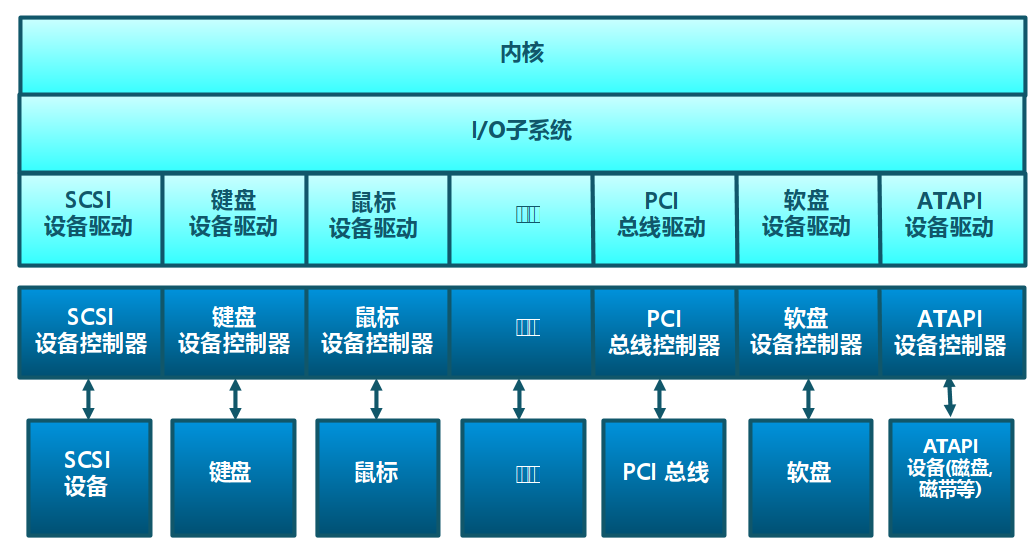
\includegraphics[width=0.8\linewidth]{figs/os-io-arch.png}
  %  \caption{xxxx}
    \end{figure}
\end{frame}

%----------------------------------------------
\begin{frame}[fragile]
    \frametitle{I/O请求生存周期}
    %    \framesubtitle{xxxx}
    %% figure
    \begin{figure}
        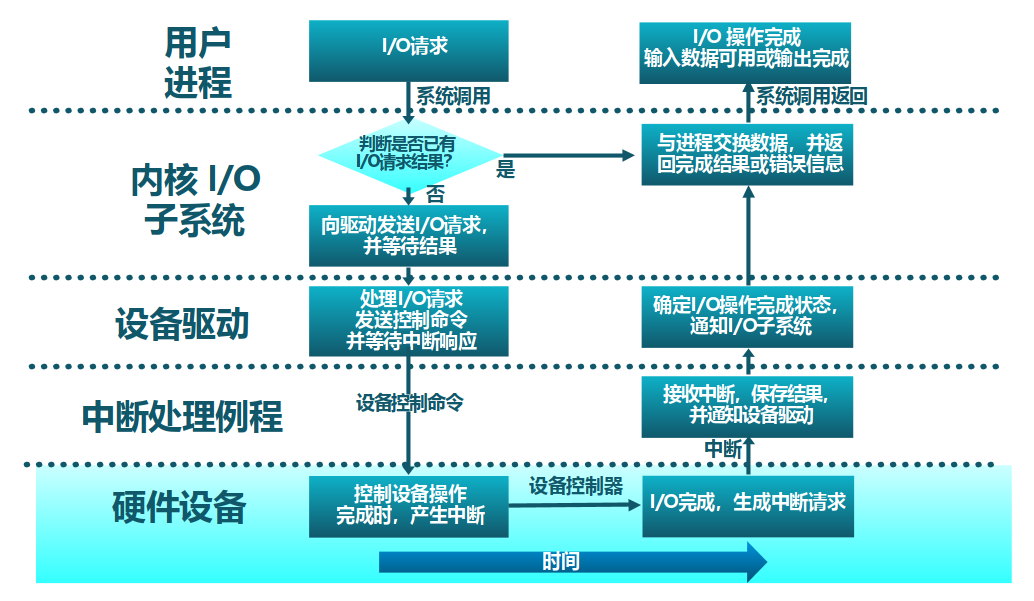
\includegraphics[width=0.8\linewidth]{figs/os-io-lifetime.png}
        %  \caption{xxxx}
    \end{figure}
\end{frame}
%----------------------------------------------
%----------------------------------------------
\begin{frame}
\frametitle{提纲} % Table of contents slide, comment this block out to remove it
\tableofcontents % Throughout your presentation, if you choose to use \section{} and \subsection{} commands, these will automatically be printed on this slide as an overview of your presentation

%% itemize
%Ref:
%    \begin{itemize}
%        \item \href{http://osq.cs.berkeley.edu/public/JFoster-Drivers.ppt}{Linux Device Drivers Overview}
%        \item \href{http://ermak.cs.nstu.ru/understanding.linux.kernel.pdf}{Understanding the Linux Kernel}
%    \end{itemize}

\end{frame}
%----------------------------------------------
\subsection{I/O设备抽象} % A subsection can be created just before a set of slides with a common theme to further break down your presentation into chunks
%----------------------------------------------
%----------------------------------------------
\begin{frame}[fragile]
    \frametitle{I/O接口的交互协议}
    %    \framesubtitle{xxxx}
    外设的两部分重要组成部分
    \begin{itemize}
        \item 对外向系统其他部分展现的设备I/O接口(hardware I/O interface)
        \item 对内的内部结构,包含了设备相关物理实现
    \end{itemize}
    \begin{figure}
    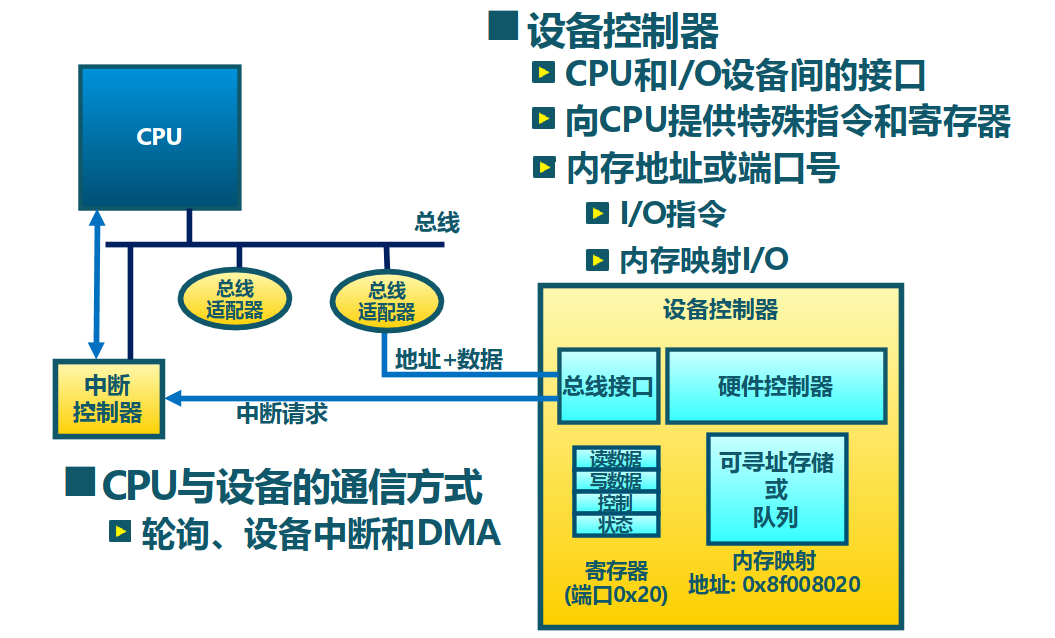
\includegraphics[width=0.5\linewidth]{figs/cpu-connect-dev.png}
    %  \caption{xxxx}
\end{figure}
\end{frame}

%----------------------------------------------
\begin{frame}[fragile]
    \frametitle{I/O接口的交互协议:基于轮询的抽象设备接口}
    %    \framesubtitle{xxxx}
    % 一个简化的抽象设备接口需要包括三部分:
    \begin{itemize}
        \item 状态
        \item 命令
        \item 数据
    \end{itemize}
    \begin{figure}
        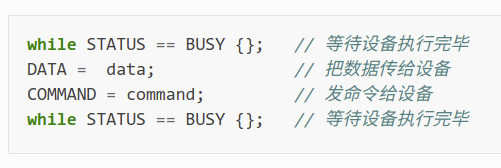
\includegraphics[width=0.7\linewidth]{figs/simple-io-interface.png}
        %  \caption{xxxx}
    \end{figure}
\end{frame}

%----------------------------------------------
\begin{frame}[fragile]
    \frametitle{I/O接口的交互协议:基于中断的抽象设备接口}
    %    \framesubtitle{xxxx}
    % 带中断机制的抽象设备接口需要包括四部分:
    \begin{itemize}
        \item 状态 / 命令 / 数据
        \item 中断
    \end{itemize}
    \begin{figure}
        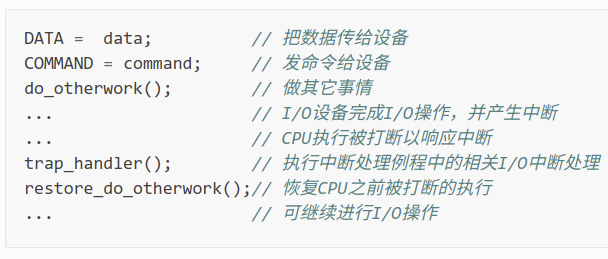
\includegraphics[width=0.7\linewidth]{figs/intr-io-interface.png}
        %  \caption{xxxx}
    \end{figure}
\end{frame}

%----------------------------------------------
\begin{frame}[fragile]
    \frametitle{设备抽象}
    %    \framesubtitle{xxxx}
    基于文件的I/O设备抽象
    \begin{itemize}
        \item 访问接口:open/close/read/write
        \item 特别的系统调用:ioctl :input/output control
        \item ioctl 系统调用很灵活,但它的问题是太灵活了,请求码的定义无规律可循
        \item 文件的接口太面向用户应用,不足覆盖到操作系统对设备进行管理的过程
    \end{itemize}

\end{frame}

%----------------------------------------------
\begin{frame}[fragile]
    \frametitle{设备抽象}
    %    \framesubtitle{xxxx}
    基于流的I/O设备抽象
    \begin{itemize}
        \item 流是用户进程和设备或伪设备之间的全双工连接
        \item 特别的系统调用:ioctl :input/output control
        \item ioctl 系统调用很灵活,但它的问题是太灵活了,请求码的定义无规律可循
        \item Dennis M. Ritchie写出了“A Stream Input-Output System”,1984
    \end{itemize}
        \begin{figure}
        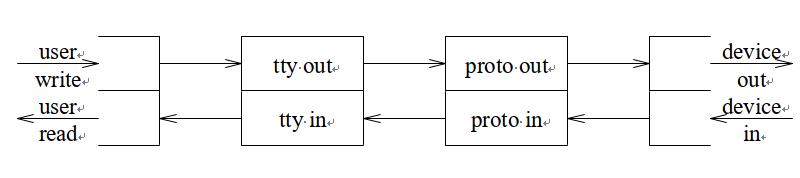
\includegraphics[width=0.7\linewidth]{figs/stream.png}
        %  \caption{xxxx}
    \end{figure}
\end{frame}

%----------------------------------------------
\begin{frame}[fragile]
    \frametitle{设备抽象}
    %    \framesubtitle{xxxx}
    基于\href{https://developer.ibm.com/technologies/linux/articles/l-virtio/}{virtio}的I/O设备抽象
    \begin{itemize}
        \item Rusty Russell在2008年提出通用I/O设备抽象 – virtio规范
        \item 虚拟机提供virtio设备的实现,virtio设备有着统一的virtio接口
        \item OS只要能够实现这些通用的接口,就可以管理和控制各种virtio设备
    \end{itemize}
    \begin{figure}
        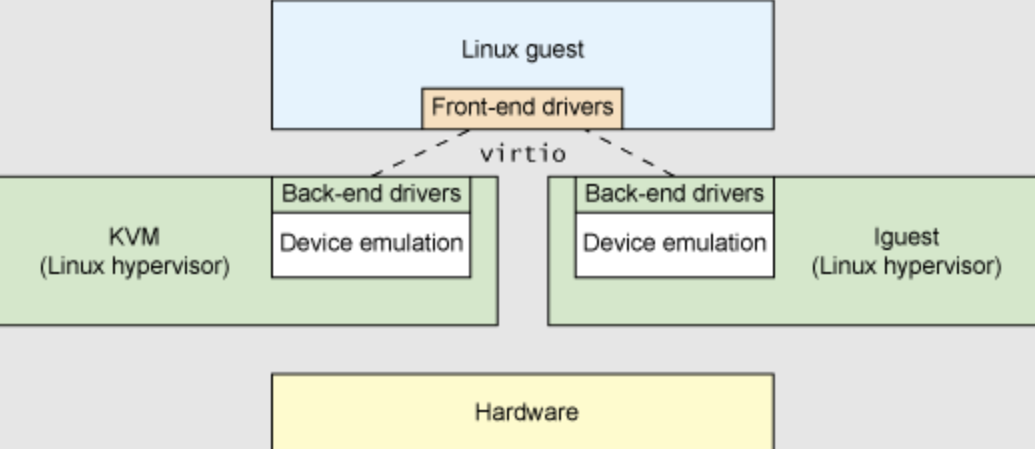
\includegraphics[width=0.6\linewidth]{figs/virtio.png}
        %  \caption{xxxx}
    \end{figure}
\end{frame}
%----------------------------------------------
\begin{frame}
\frametitle{提纲} % Table of contents slide, comment this block out to remove it
\tableofcontents % Throughout your presentation, if you choose to use \section{} and \subsection{} commands, these will automatically be printed on this slide as an overview of your presentation

%% itemize
%Ref:
%    \begin{itemize}
%        \item \href{http://osq.cs.berkeley.edu/public/JFoster-Drivers.ppt}{Linux Device Drivers Overview}
%        \item \href{http://ermak.cs.nstu.ru/understanding.linux.kernel.pdf}{Understanding the Linux Kernel}
%    \end{itemize}

\end{frame}
%----------------------------------------------
\subsection{I/O执行模型} % A subsection can be created just before a set of slides with a common theme to further break down your presentation into chunks
%----------------------------------------------
%----------------------------------------------
\begin{frame}[fragile]
    \frametitle{I/O执行模型}
    %    \framesubtitle{xxxx}
    I/O执行模型
    \begin{itemize}
        \item 用户进程是通过I/O相关的系统调用来进行I/O操作的
        \item 大致可以分为五种I/O执行模型(I/O Model, I/O模型)
        \begin{itemize}
            \item blocking I/O
            \item nonblocking I/O
            \item I/O multiplexing
            \item signal driven I/O
            \item asynchronous I/O
        \end{itemize}
    \end{itemize}
%    \begin{figure}
%        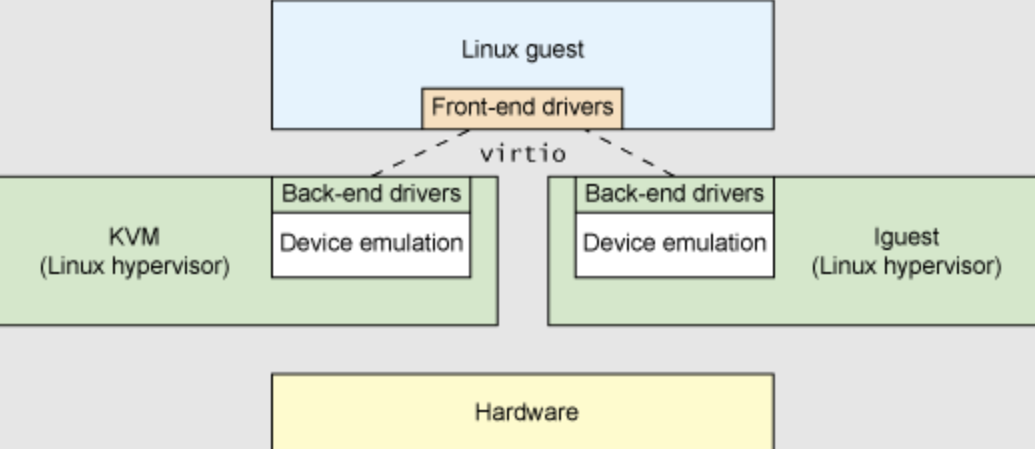
\includegraphics[width=0.6\linewidth]{figs/virtio.png}
%        %  \caption{xxxx}
%    \end{figure}
\end{frame}

%----------------------------------------------
\begin{frame}[fragile]
    \frametitle{I/O执行模型}
    %    \framesubtitle{xxxx}
    当一个用户进程发出一个 read I/O系统调用时,主要经历两个阶段:
    \begin{itemize}
        \item 1. 等待数据准备好 
        \item 2. 把数据从内核拷贝到用户进程中
     \end{itemize}       
    如果关注的是进程的执行状态
        \begin{itemize}
            \item 阻塞:进程执行系统调用后会被阻塞
            \item 非阻塞:进程执行系统调用后不会被阻塞
        \end{itemize}

    %    \begin{figure}
    %        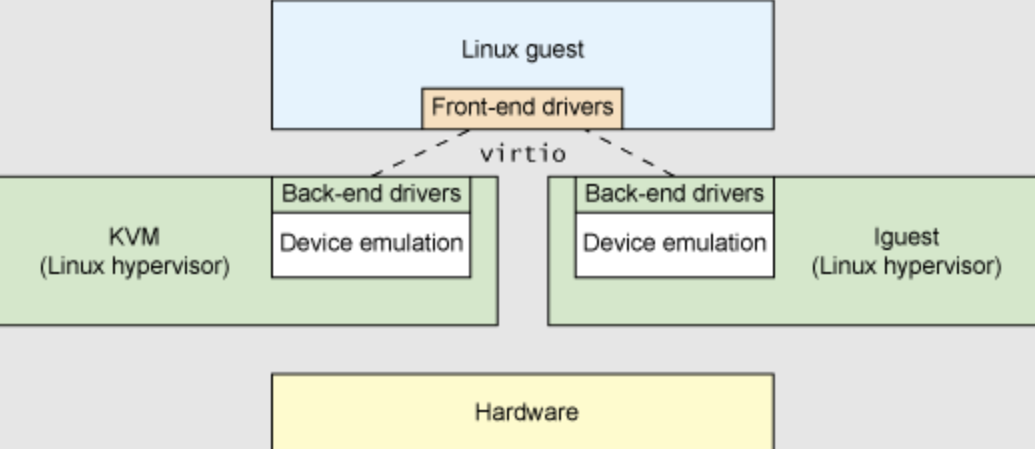
\includegraphics[width=0.6\linewidth]{figs/virtio.png}
    %        %  \caption{xxxx}
    %    \end{figure}
\end{frame}
%----------------------------------------------
\begin{frame}[fragile]
    \frametitle{I/O执行模型}
    %    \framesubtitle{xxxx}
    当一个用户进程发出一个 read I/O系统调用时,主要经历两个阶段:
    \begin{itemize}
        \item 1. 等待数据准备好 
        \item 2. 把数据从内核拷贝到用户进程中
    \end{itemize}       
    如果关注的是消息通信机制
    \begin{itemize}
        \item 同步:用户进程与操作系统之间的操作是经过双方协调的,步调一致的
        \item 异步:用户进程与操作系统之间并不需要协调,都可以随意进行各自的操作
    \end{itemize}
    
    %    \begin{figure}
    %        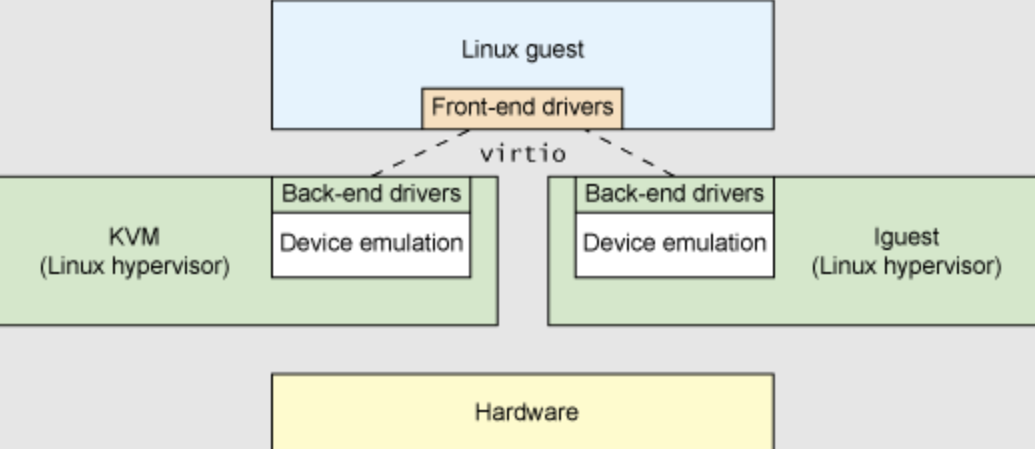
\includegraphics[width=0.6\linewidth]{figs/virtio.png}
    %        %  \caption{xxxx}
    %    \end{figure}
\end{frame}

%----------------------------------------------
\begin{frame}[fragile]
    \frametitle{I/O执行模型:阻塞I/O}
    %    \framesubtitle{xxxx}
    基于阻塞I/O(blocking I/O)模型的文件读系统调用 – read 的执行过程是:
    \begin{enumerate}

        \item 用户进程发出 read 系统调用;
        \item 内核发现所需数据没在I/O缓冲区中,需要向磁盘驱动程序发出I/O操作,并让用户进程处于阻塞状态;
        \item 磁盘驱动程序把数据从磁盘传到I/O缓冲区后,通知内核(一般通过中断机制),内核会把数据从I/O缓冲区拷贝到用户进程的buffer中,并唤醒用户进程(即用户进程处于就绪态);
        \item 内核从内核态返回到用户态的用户态进程,此时 read 系统调用完成。
    \end{enumerate}       

    所以阻塞I/O(blocking IO)的特点就是用户进程在I/O执行的两个阶段(等待数据和拷贝数据两个阶段)都是阻塞的。
    
    %    \begin{figure}
    %        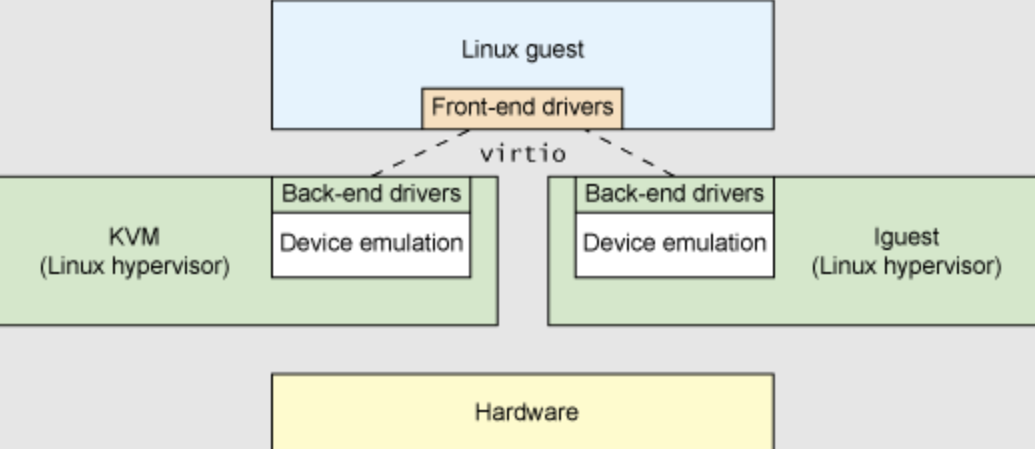
\includegraphics[width=0.6\linewidth]{figs/virtio.png}
    %        %  \caption{xxxx}
    %    \end{figure}
\end{frame}
%----------------------------------------------
%----------------------------------------------
\begin{frame}[fragile]
    \frametitle{I/O执行模型:阻塞I/O}
    %    \framesubtitle{xxxx}
    % 阻塞I/O(blocking I/O)
    \begin{figure}
        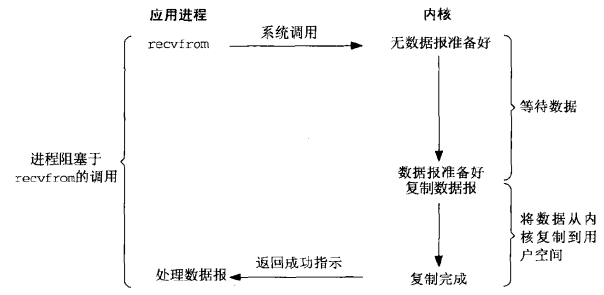
\includegraphics[width=0.85\linewidth]{figs/block-io.png}
        %  \caption{xxxx}
    \end{figure}
\end{frame}
%----------------------------------------------
\begin{frame}[fragile]
    \frametitle{I/O执行模型:非阻塞I/O}
    %    \framesubtitle{xxxx}
    基于非阻塞IO(non-blocking I/O)模型的文件读系统调用 – read 的执行过程:
    \begin{enumerate}
        
        \item 用户进程发出 read 系统调用;
        \item 内核发现所需数据没在I/O缓冲区中,需要向磁盘驱动程序发出I/O操作,并不会让用户进程处于阻塞状态,而是立刻返回一个error;
        \item 用户进程判断结果是一个error时,它就知道数据还没有准备好,于是它可以再次发送read操作(这一步操作可以重复多次);
        \item 磁盘驱动程序把数据从磁盘传到I/O缓冲区后,通知内核(一般通过中断机制),内核在收到通知且再次收到了用户进程的system call后,会马上把数据从I/O缓冲区拷贝到用户进程的buffer中;
        \item 内核从内核态返回到用户态的用户态进程,此时 read 系统调用完成。
    \end{enumerate}       
    
    所以,在非阻塞式I/O的特点是用户进程不会被内核阻塞,而是需要不断的主动询问内核所需数据准备好了没有。
    
    %    \begin{figure}
    %        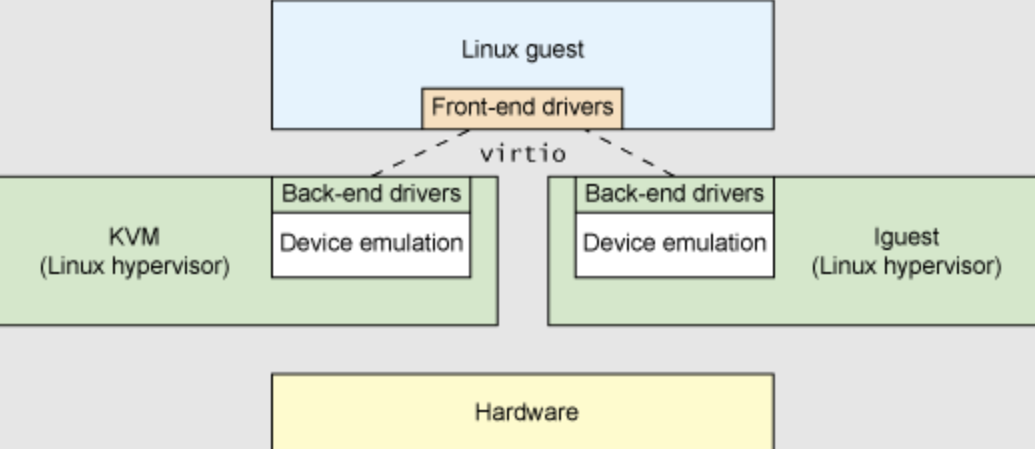
\includegraphics[width=0.6\linewidth]{figs/virtio.png}
    %        %  \caption{xxxx}
    %    \end{figure}
\end{frame}
%----------------------------------------------
\begin{frame}[fragile]
    \frametitle{I/O执行模型:非阻塞I/O}
    %    \framesubtitle{xxxx}
    % 非阻塞I/O(non-blocking I/O)
    \begin{figure}
        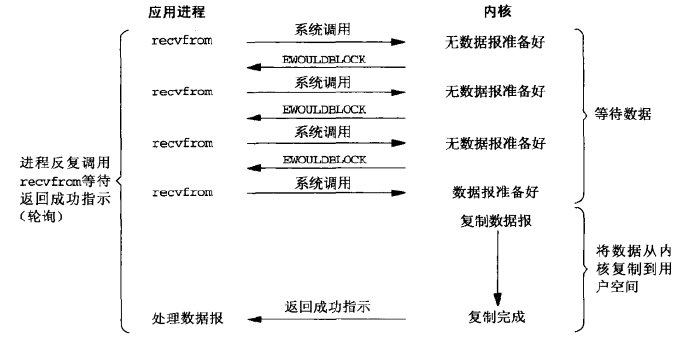
\includegraphics[width=0.8\linewidth]{figs/nonblock-io.png}
        %  \caption{xxxx}
    \end{figure}
\end{frame}
%----------------------------------------------
\begin{frame}[fragile]
    \frametitle{I/O执行模型:多路复用I/O}
    %    \framesubtitle{xxxx}
    多路复用I/O(I/O multiplexing)的文件读系统调用 – read 的执行过程:
    \begin{enumerate}
        \item 对应的I/O系统调用是 select 和 epoll 等    
        \item 通过 select 或 epoll 系统调用来不断的轮询用户进程关注的所有文件句柄或socket,当某个文件句柄或socket有数据到达了,select 或 epoll 系统调用就会返回到用户进程,用户进程再调用 read 系统调用,让内核将数据从内核的I/O缓冲区拷贝到用户进程的buffer中。
    \end{enumerate}       
    

    
    %    \begin{figure}
    %        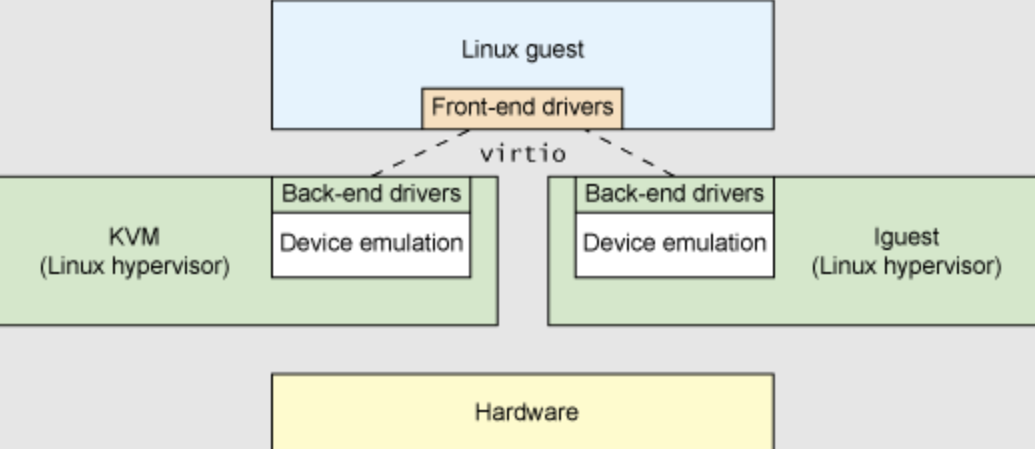
\includegraphics[width=0.6\linewidth]{figs/virtio.png}
    %        %  \caption{xxxx}
    %    \end{figure}
\end{frame}
%----------------------------------------------
\begin{frame}[fragile]
    \frametitle{I/O执行模型:多路复用I/O}
    %    \framesubtitle{xxxx}
    % 多路复用IO(signal driven I/O)
    \begin{figure}
        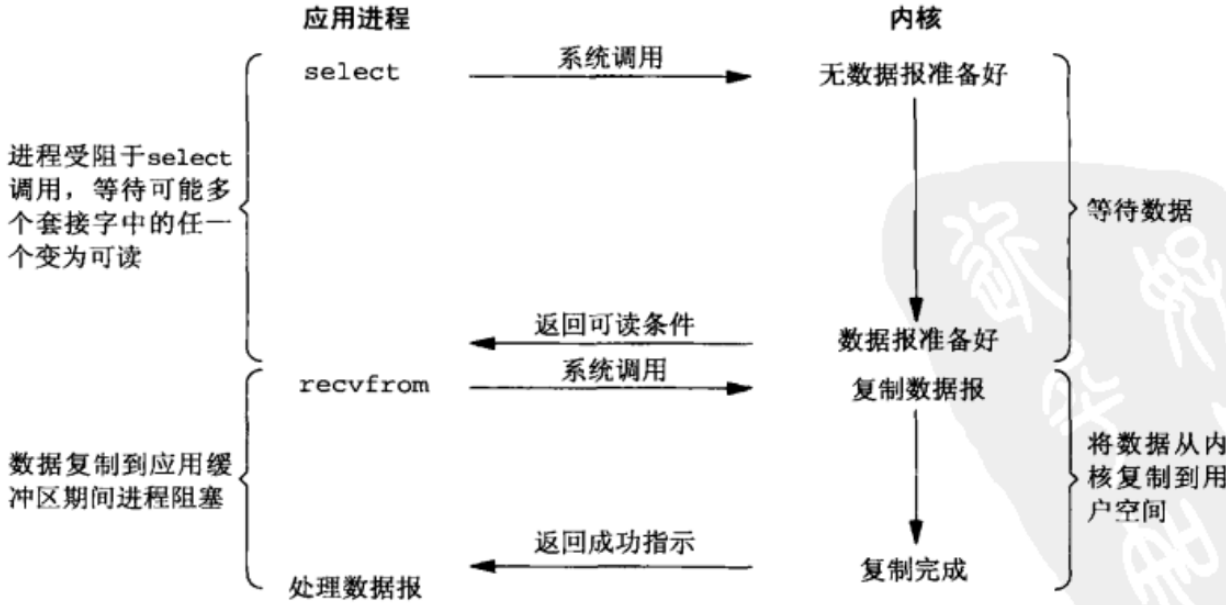
\includegraphics[width=0.8\linewidth]{figs/multi-io.png}
        %  \caption{xxxx}
    \end{figure}
\end{frame}
%----------------------------------------------
\begin{frame}[fragile]
    \frametitle{I/O执行模型:信号驱动I/O(signal driven I/O)}
    %    \framesubtitle{xxxx}
    \begin{enumerate}
\item 当进程发出一个 read 系统调用时,会向内核注册一个信号处理函数,然后系统调用返回,进程不会被阻塞,而是继续执行。
\item 当内核中的IO数据就绪时,会发送一个信号给进程,进程便在信号处理函数中调用IO读取数据。
    \end{enumerate}
    此模型的特点是,采用了回调机制,这样开发和调试应用的难度加大。 
    
    %    \begin{figure}
    %        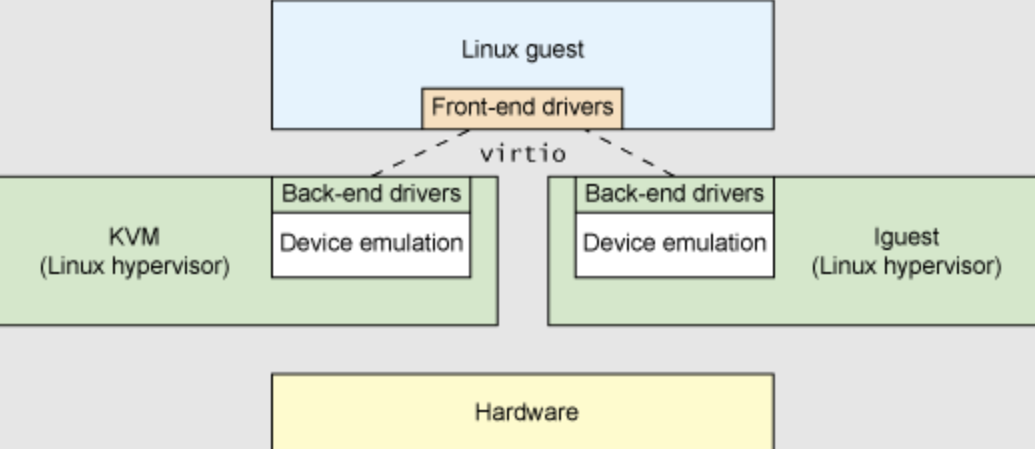
\includegraphics[width=0.6\linewidth]{figs/virtio.png}
    %        %  \caption{xxxx}
    %    \end{figure}
\end{frame}
%----------------------------------------------
\begin{frame}[fragile]
    \frametitle{I/O执行模型:信号驱动I/O}
    %    \framesubtitle{xxxx}
    % 信号驱动IO(signal driven I/O)
    \begin{figure}
        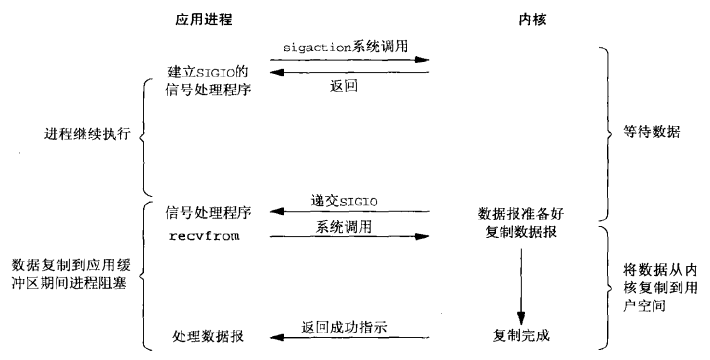
\includegraphics[width=0.8\linewidth]{figs/signal-io.png}
        %  \caption{xxxx}
    \end{figure}
\end{frame}
%----------------------------------------------
\begin{frame}[fragile]
    \frametitle{I/O执行模型:异步I/O(Asynchronous I/O)}
    %    \framesubtitle{xxxx}
    \begin{enumerate}
    \item 用户进程发起 read 异步系统调用之后,立刻就可以开始去做其它的事。
    \item 从内核的角度看,当它收到一个 read 异步系统调用之后,首先它会立刻返回,所以不会对用户进程产生任何阻塞情况。
    \item kernel会等待数据准备完成,然后将数据拷贝到用户内存。
    \item 当这一切都完成之后,kernel会通知用户进程,告诉它read操作完成了。
    \end{enumerate}    
    
    
    %    \begin{figure}
    %        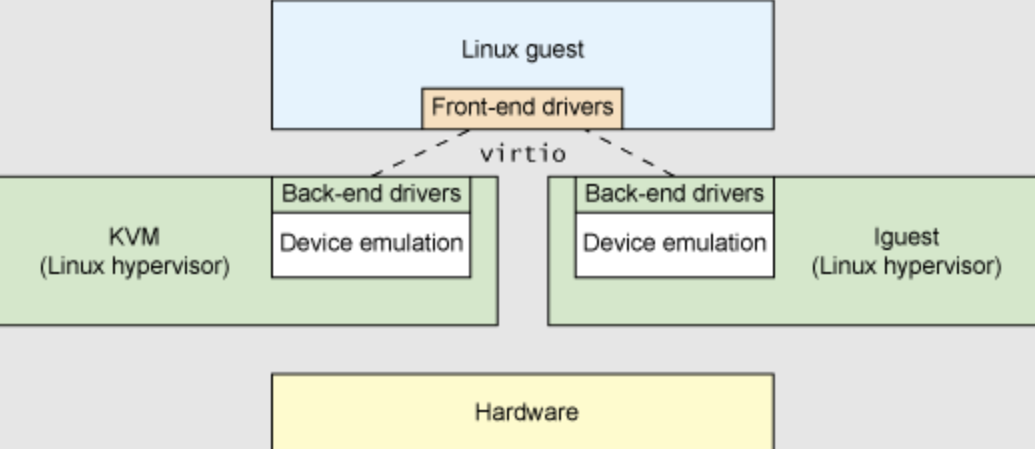
\includegraphics[width=0.6\linewidth]{figs/virtio.png}
    %        %  \caption{xxxx}
    %    \end{figure}
\end{frame}

%----------------------------------------------
\begin{frame}[fragile]
    \frametitle{I/O执行模型:异步I/O}
    %    \framesubtitle{xxxx}
    % 异步IO
    \begin{figure}
        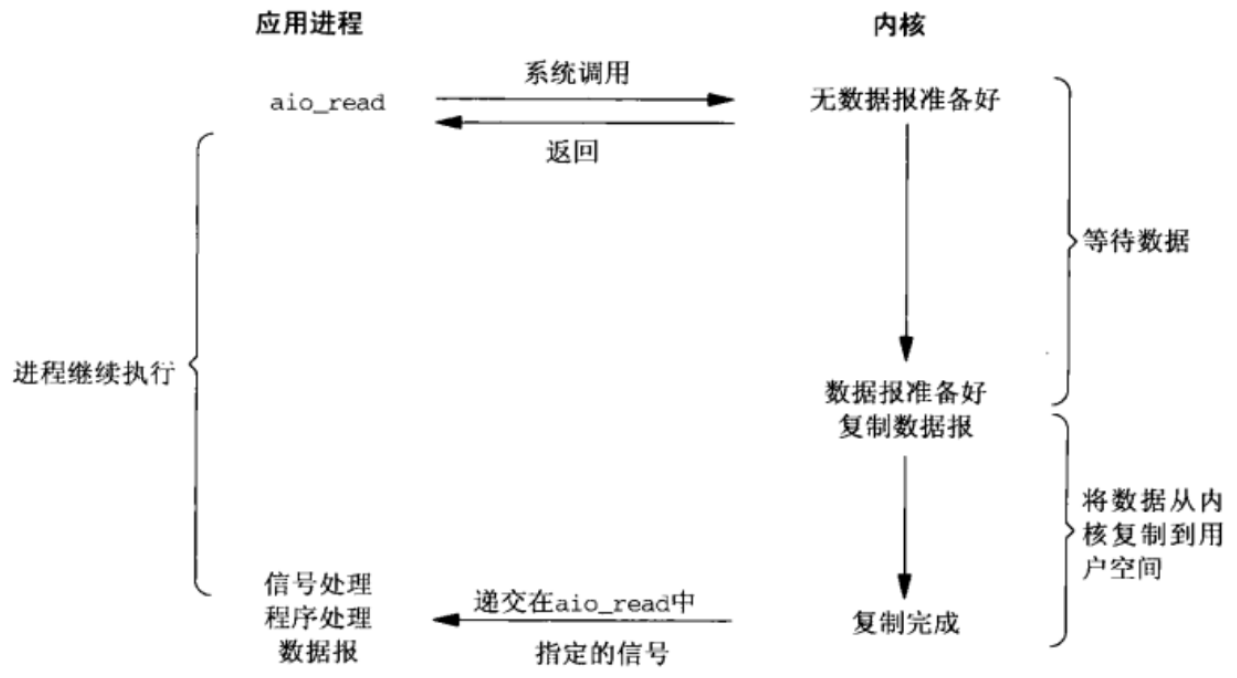
\includegraphics[width=0.8\linewidth]{figs/async-io.png}
        %  \caption{xxxx}
    \end{figure}
\end{frame}
%----------------------------------------------
\begin{frame}[fragile]
    \frametitle{I/O执行模型:五种I/O执行模型对比}
    %    \framesubtitle{xxxx}
    % 五种I/O执行模型对比
    
    \begin{enumerate}
        
        \item 阻塞I/O:在用户进程发出I/O系统调用后,进程会等待该IO操作完成,而使得进程的其他操作无法执行。
        \item 非阻塞I/O:在用户进程发出I/O系统调用后,如果数据没准备好,该I/O操作会立即返回,之后进程可以进行其他操作;如果数据准备好了,用户进程会通过系统调用完成数据拷贝并接着进行数据处理。
        \item 多路复用I/O:将多个非阻塞I/O请求的轮询操作合并到一个select或epoll系统调用中进行。
        \item 信号驱动I/O:利用信号机制完成从内核到应用进程的事件通知。
        \item 异步I/O:不会导致请求进程阻塞。
    \end{enumerate}       
    
    % 从上述分析可以得知,阻塞和非阻塞的区别在于内核数据还没准备好时,用户进程是否会阻塞(一阶段是否阻塞);同步与异步的区别在于当数据从内核copy到用户空间时,用户进程是否会阻塞/参与(二阶段是否阻塞)。
    
    %    \begin{figure}
    %        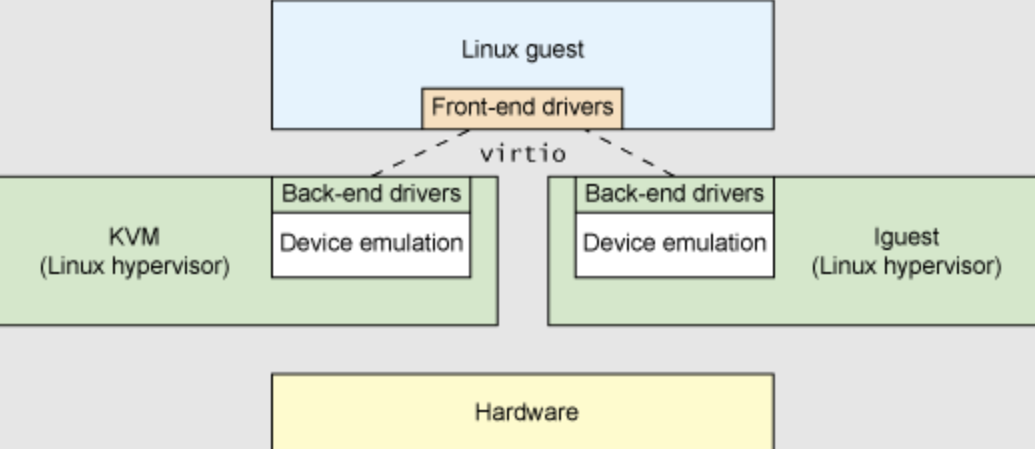
\includegraphics[width=0.6\linewidth]{figs/virtio.png}
    %        %  \caption{xxxx}
    %    \end{figure}
\end{frame}
%----------------------------------------------
\begin{frame}[fragile]
    \frametitle{I/O执行模型}
    %    \framesubtitle{xxxx}
      五种IO执行模型对比
    \begin{figure}
        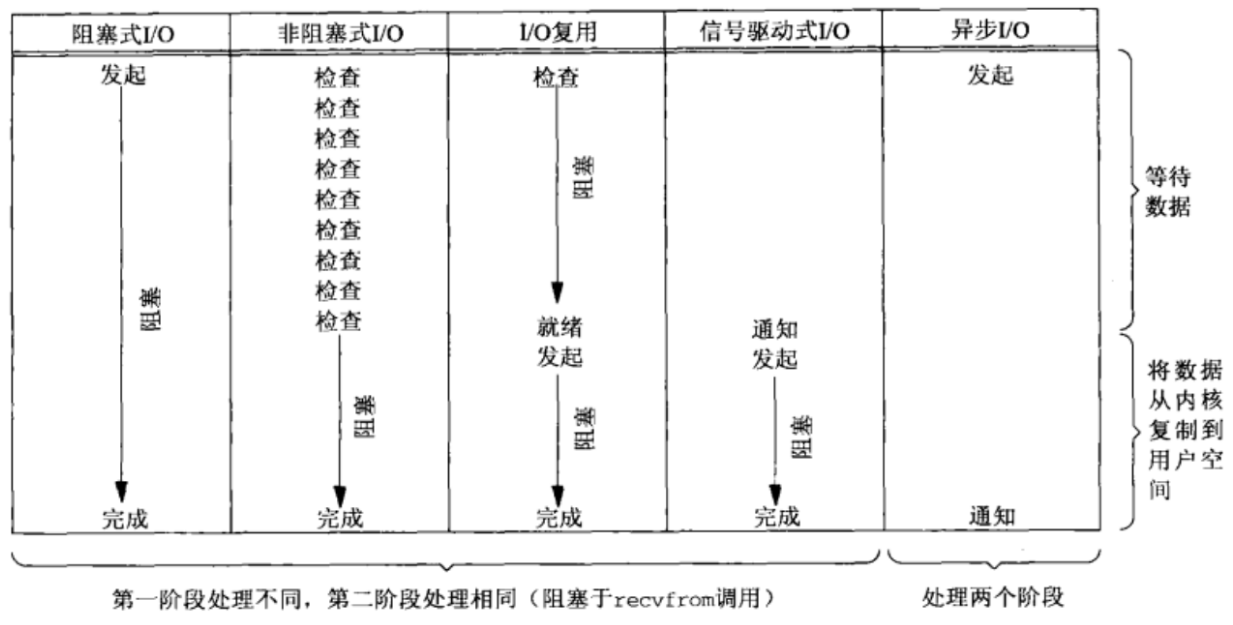
\includegraphics[width=0.8\linewidth]{figs/io-modes-compare.png}
        %  \caption{xxxx}
    \end{figure}
\end{frame}
%----------------------------------------------
\end{document}
